\chapter{Introduction}
\noindent
\rule{\textwidth}{0.4pt}

\begin{center}
\begin{minipage}{0.8\textwidth}
\textit{In Chapter 1, the authors provide a comprehensive introduction to the project’s domain, presenting the relevant background and context. Based on this overview, the problem statement is carefully formulated, emphasizing its significance, scope, and the main objectives that the project aims to achieve.}
\end{minipage}
\end{center}

\section{Problem statement}

With the rapid progress in educational technology, the concept of an online coding platform with a ranking system for students is increasingly recognized as a valuable tool to enhance learning outcomes, foster problem-solving skills as well as serving as a solid foundation to prepare students for real-world job interviews in the labor market. While some recognized global platforms such as LeetCode and Codeforces provide extensive resources for competitive programming, there remains a gap in platforms tailored specifically to the needs of Vietnamese students. Current solutions do not fully address the language preferences, localized content, or the collaborative opportunities required to create a holistic learning environment. Consequently, it is essential to enhance the manner in which students approach coding problems, submit their solutions, and collaborate with peers in an effective and intuitive way.

One of the primary challenges lies in problem management and submission tracking. Students require a system that allows them to browse coding problems by category and difficulty, submit solutions with immediate evaluation, and track their performance over time. The lack of a structured and interactive ranking mechanism can reduce motivation and hinder continuous improvement, as students may struggle to assess their progress and compare their performance with peers effectively.

Another significant challenge is fostering real-time collaboration and discussion. Existing platforms often lack localized forums where students can post questions, discuss problem-solving strategies, and exchange knowledge in their own language. Without an integrated discussion system, students may confront barriers in clarifying ambiguities and engage in collaborative learning, which significantly curtails both overall engagement and the depth of the learning experience.

In summary, the system must be accessible and intuitive, catering to students with various levels of programming expertise. By offering a user-friendly interface, real-time submission feedback, a ranking system, and an integrated discussion forum, the platform can foster an interactive and engaging environment. This approach encourages students to actively participate, receive immediate feedback on their work, and collaborate effectively with their peers, thereby enhancing the overall learning experience. These challenges highlight the necessity of a system designed specifically for Vietnamese students that integrates problem-solving, submission tracking, and collaborative learning in a seamless manner.

\section{Goals}

The main goal of this project is to design and implement a Code Ranking System specifically tailored for Vietnamese students, addressing the challenges identified in the problem statement. The system aims to provide an intuitive and accessible platform that allows undergraduates to effectively engage with coding problems, submit solutions, and interact with their peers. By focusing on usability and real-time feedback, the platform seeks to enhance learning outcomes and foster a collaborative environment.

Firstly, the system will enable students to browse coding problems organized by category and difficulty level, with clear description and examples. Students will be able to submit their solutions and receive immediate evaluation, allowing them to track their progress and monitor improvement over time. A structured ranking mechanism will provide motivation and encourage healthy competition among users.

Secondly, the platform will incorporate real-time centralized discussion features,  where students can post questions, share strategies, and collaborate with peers in their native language. This will help clarify ambiguities, promote knowledge sharing, and deepen the learning experience.

Thirdly, the platform will provide a free chatbot feature that allows students to ask questions and engage with the bot regarding topics relevant to coding, problem-solving, and real-world interview scenarios in the Vietnamese job market. This chatbot aims to simulate practical interview discussions, offer guidance, and help students prepare for professional opportunities.

Finally, the platform will support teachers and moderators with administrative functionalities. These include problem management, monitoring student submissions, and generating performance statistics, thereby providing insights to improve teaching strategies and maintain a structured, high-quality learning environment.

In summary, this project aims to create an interactive, motivating, and collaborative coding platform for Vietnamese students, facilitating skill development, real-time feedback, peer engagement, and practical interview preparation, while bridging the gap between global competitive programming platforms and the local educational context.

\section{Scope}

Our team is developing a web-based platform specifically designed for desktop users, integrating AI-driven features to enhance the learning and coding experience.

\begin{itemize}
    \item \textbf{Website:} By focusing on PC compatibility, the platform ensures smooth navigation and interaction for students. Key modules include problem exploration, solution submission, ranking system, and a centralized discussion forum where students can engage, share insights, and collaborate.
    \item \textbf{AI-powered Assistance:} The system incorporates an intelligent chatbot that helps students with coding guidance and interview preparation. Using natural language processing, the chatbot can interpret questions and provide personalized recommendations, enabling students to improve their skills and gain practical experience in preparing for real-world job opportunities.
\end{itemize}

To ensure feasibility and maintain a well-defined development focus, the scope of the platform is further clarified through the following technical and functional limitations.

\subsection*{Supported Programming Languages}

The platform initially supports a limited number of programming languages that are widely used in Vietnamese universities and commonly required in technical interviews. These languages include \textbf{C\#}, \textbf{Java} and \textbf{Python}. This selection ensures compatibility with academic curricula while simplifying the implementation of the automated judging system. Support for additional programming languages is considered outside the scope of the current project phase.

\subsection*{Problem Types and Algorithm Coverage}

The platform focuses on fundamental and intermediate-level algorithmic problems that are essential for developing core problem-solving skills. The supported problem categories include:
\begin{itemize}
    \item Basic programming concepts and mathematical problems
    \item Array and string manipulation
    \item Searching and sorting algorithms
    \item Introductory to intermediate-level dynamic programming
\end{itemize}

Advanced topics such as machine learning algorithms, distributed systems, or highly specialized competitive programming techniques are explicitly excluded from the project scope.

\subsection*{Contest and Evaluation Scope}

The platform supports individual-based practice sessions as well as live programming contests with real-time multiplayer participation, allowing multiple users to compete simultaneously under the same problem set and time constraints. All code submissions are evaluated automatically using predefined test cases with standard time and memory limits to ensure consistency and fairness in assessment. However, the system does not support team-based contests, and advanced plagiarism detection mechanisms are excluded from the current project scope.
\subsection*{Platform Constraints}

The system is optimized exclusively for desktop web browsers to ensure stable performance and a consistent user experience. Mobile device support, native applications, and offline usage are beyond the scope of this project. Additionally, the platform focuses on educational and practice-oriented functionalities rather than serving as a full-scale commercial competitive programming system.

By clearly defining these boundaries, the project maintains a realistic and manageable scope while effectively addressing the learning needs of Vietnamese IT students in algorithm practice and programming contest preparation.

\section{Related works}
\subsection{Leetcode}

\begin{figure}[h!]
    \centering
    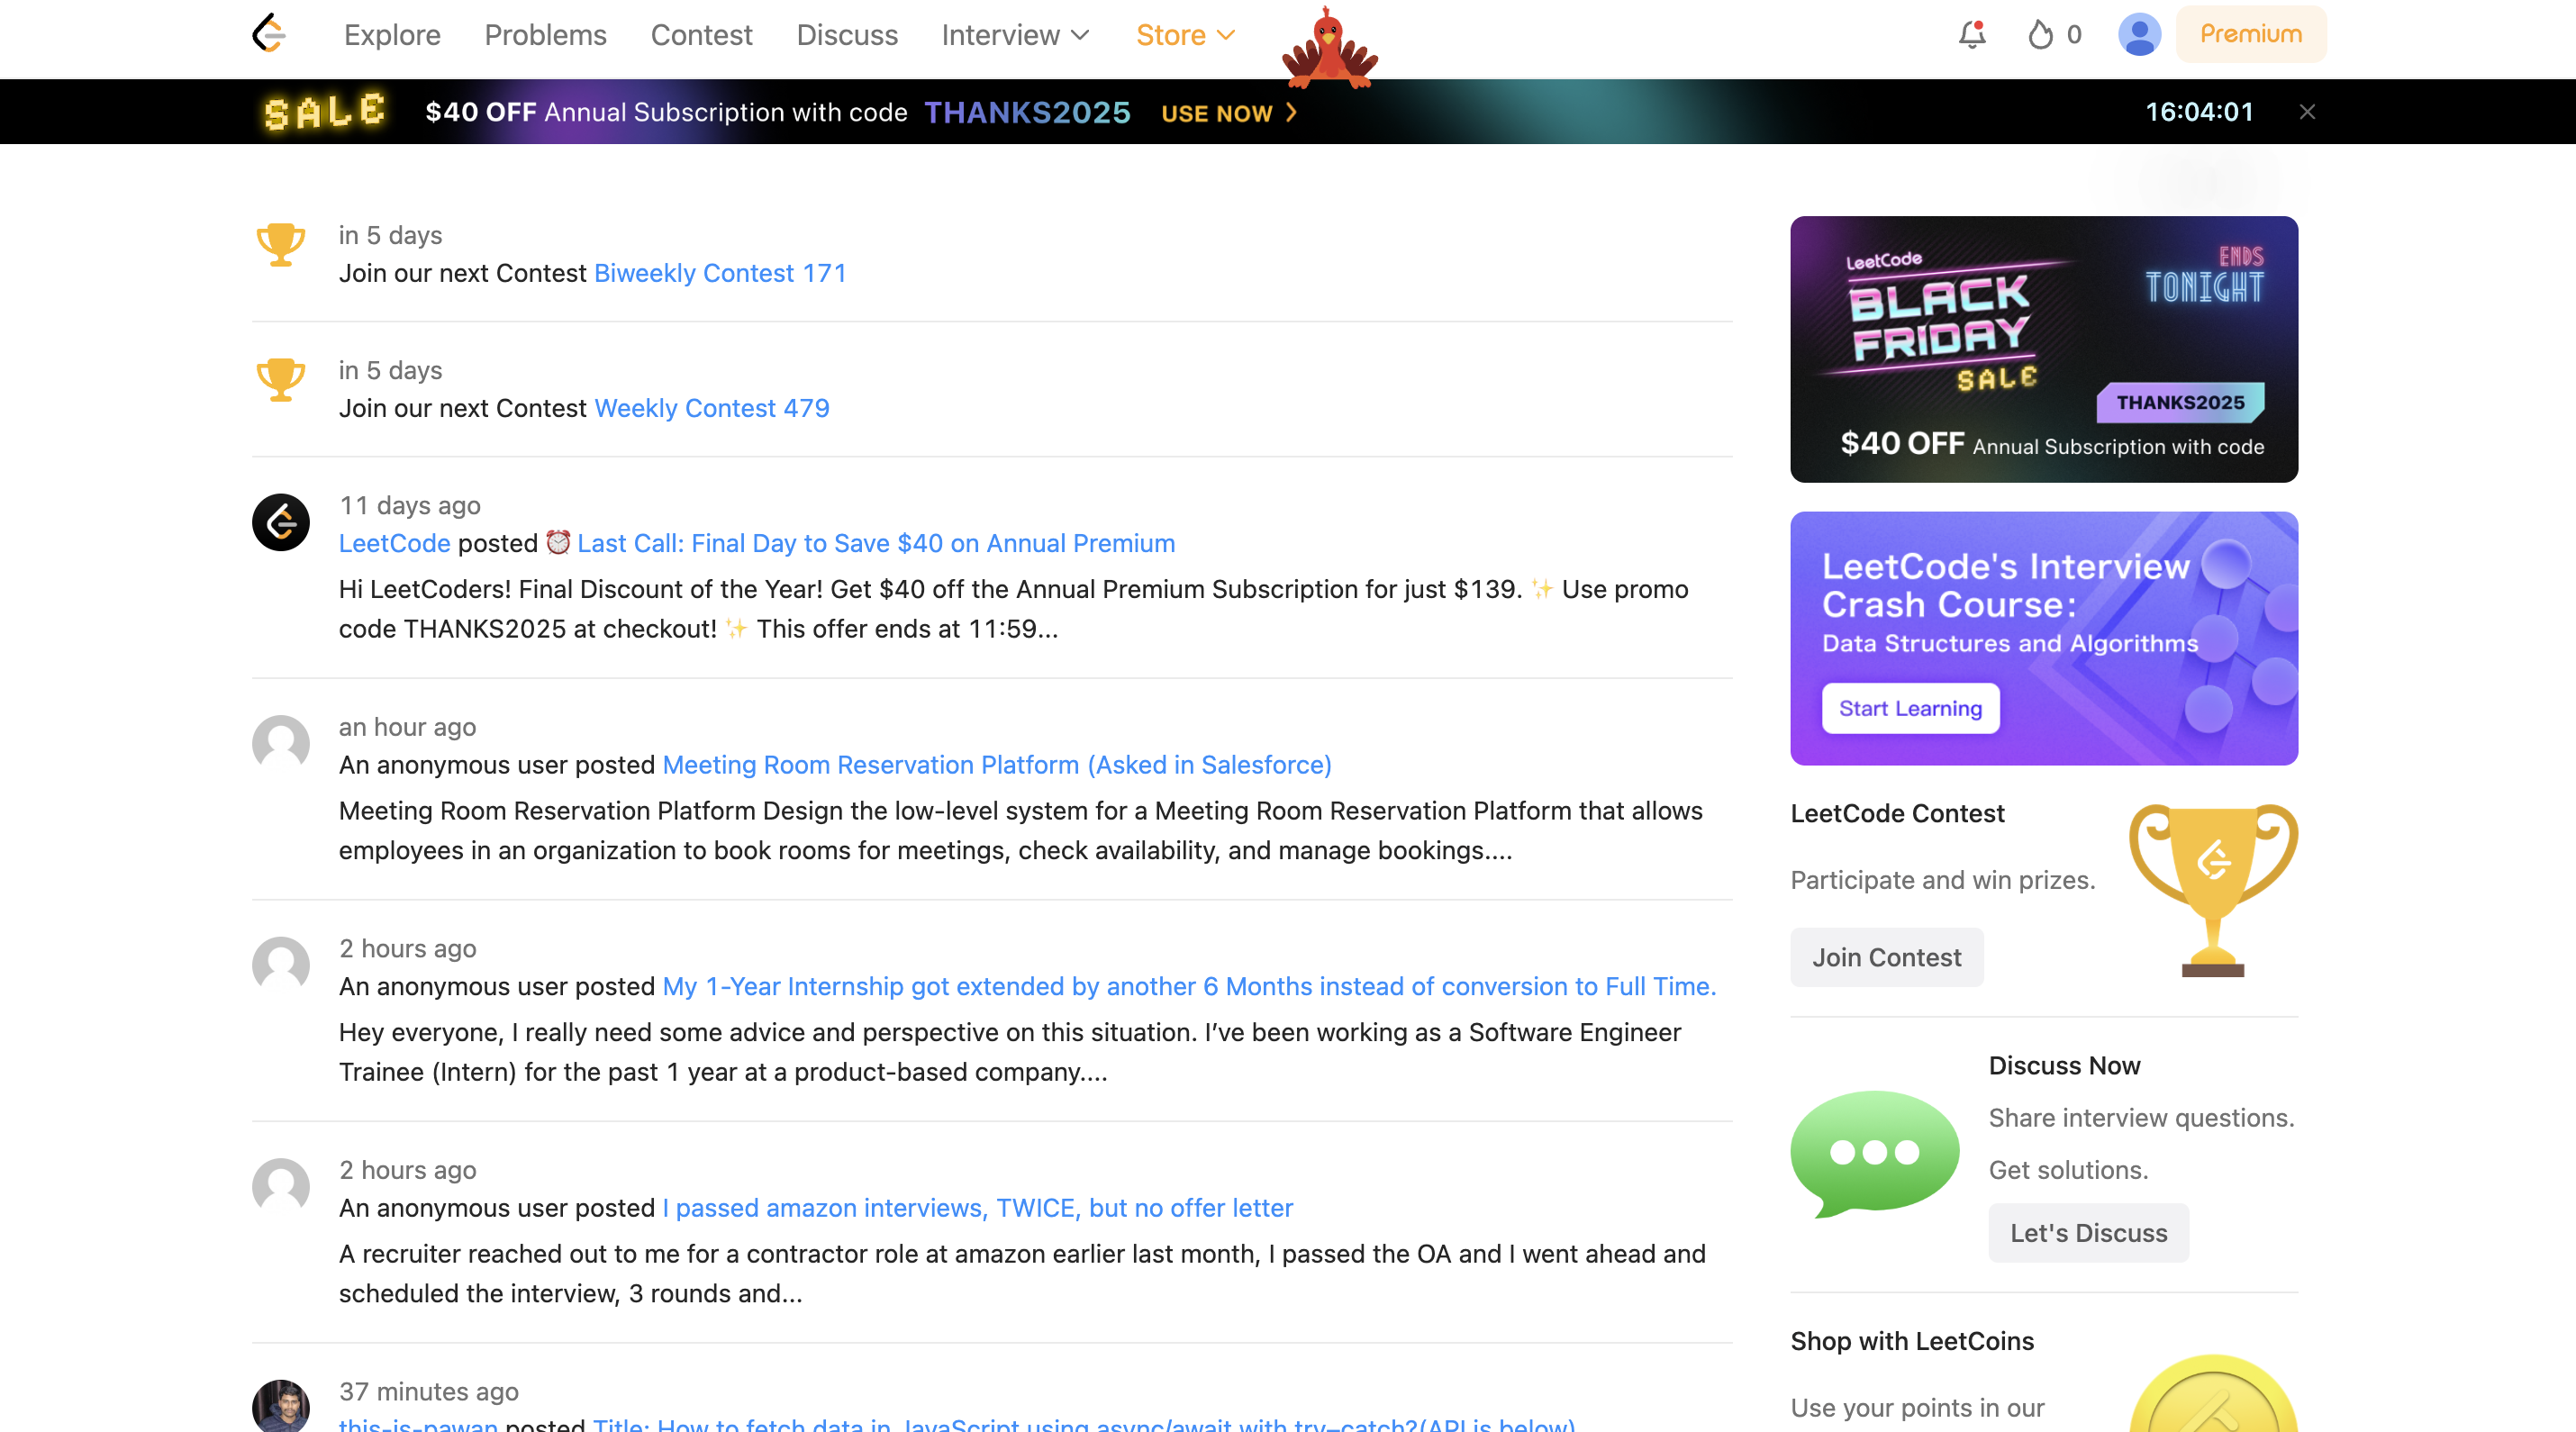
\includegraphics[width=1\textwidth]{Contents/Chapter 1/Images/Leetcode.png}
    \vspace{0.6cm}
    \caption{Leetcode Homepage}
    \label{fig:leetcode-system}
\end{figure}

LeetCode, founded in 2015 based on the co-founders’ experiences working at Google and Amazon, has become a highly popular online coding platform that offers a large collection of programming problems for all skill levels. It offers a comprehensive environment where users can practice a wide variety of programming problems, engage with a global community, and track their progress over time.LeetCode is widely recognized for its role in fostering problem-solving abilities and strengthening algorithmic thinking, making it an essential tool for both students and professionals in the software engineering field.\\

Key features of LeetCode include:
\begin{itemize}
    \item \textbf{Extensive Problem Library:} Thousands of coding problems across multiple difficulty levels and topics.
    \item \textbf{Online Code Editor:} Supports multiple programming languages with instant feedback and test case evaluation.
    \item \textbf{Contest and Challenge System:} Regular coding contests to benchmark skills against a global community.
    \item \textbf{Interview Preparation Kits:} Curated problem sets designed to prepare users for technical interviews at top tech companies.
    \item \textbf{Discussion Forums:} Active community discussions for problem-solving strategies, solutions, and learning resources.
    \item \textbf{Progress Tracking and Analytics:} Tools to monitor performance, problem-solving patterns, and skill improvement over time.
\end{itemize}

LeetCode offers a diverse set of core features that comprehensively address the needs of different user roles, including problem solving, submission tracking, contest participation, community interaction, ranking, and interview preparation. These features collectively enhance the learning experience, promote skill development, and encourage active engagement within the platform. However, it is noteworthy that LeetCode currently does not provide a public leaderboard to foster a stronger competitive environment among users.
\subsection{Codeforces}

\begin{figure}[h!]
    \centering
    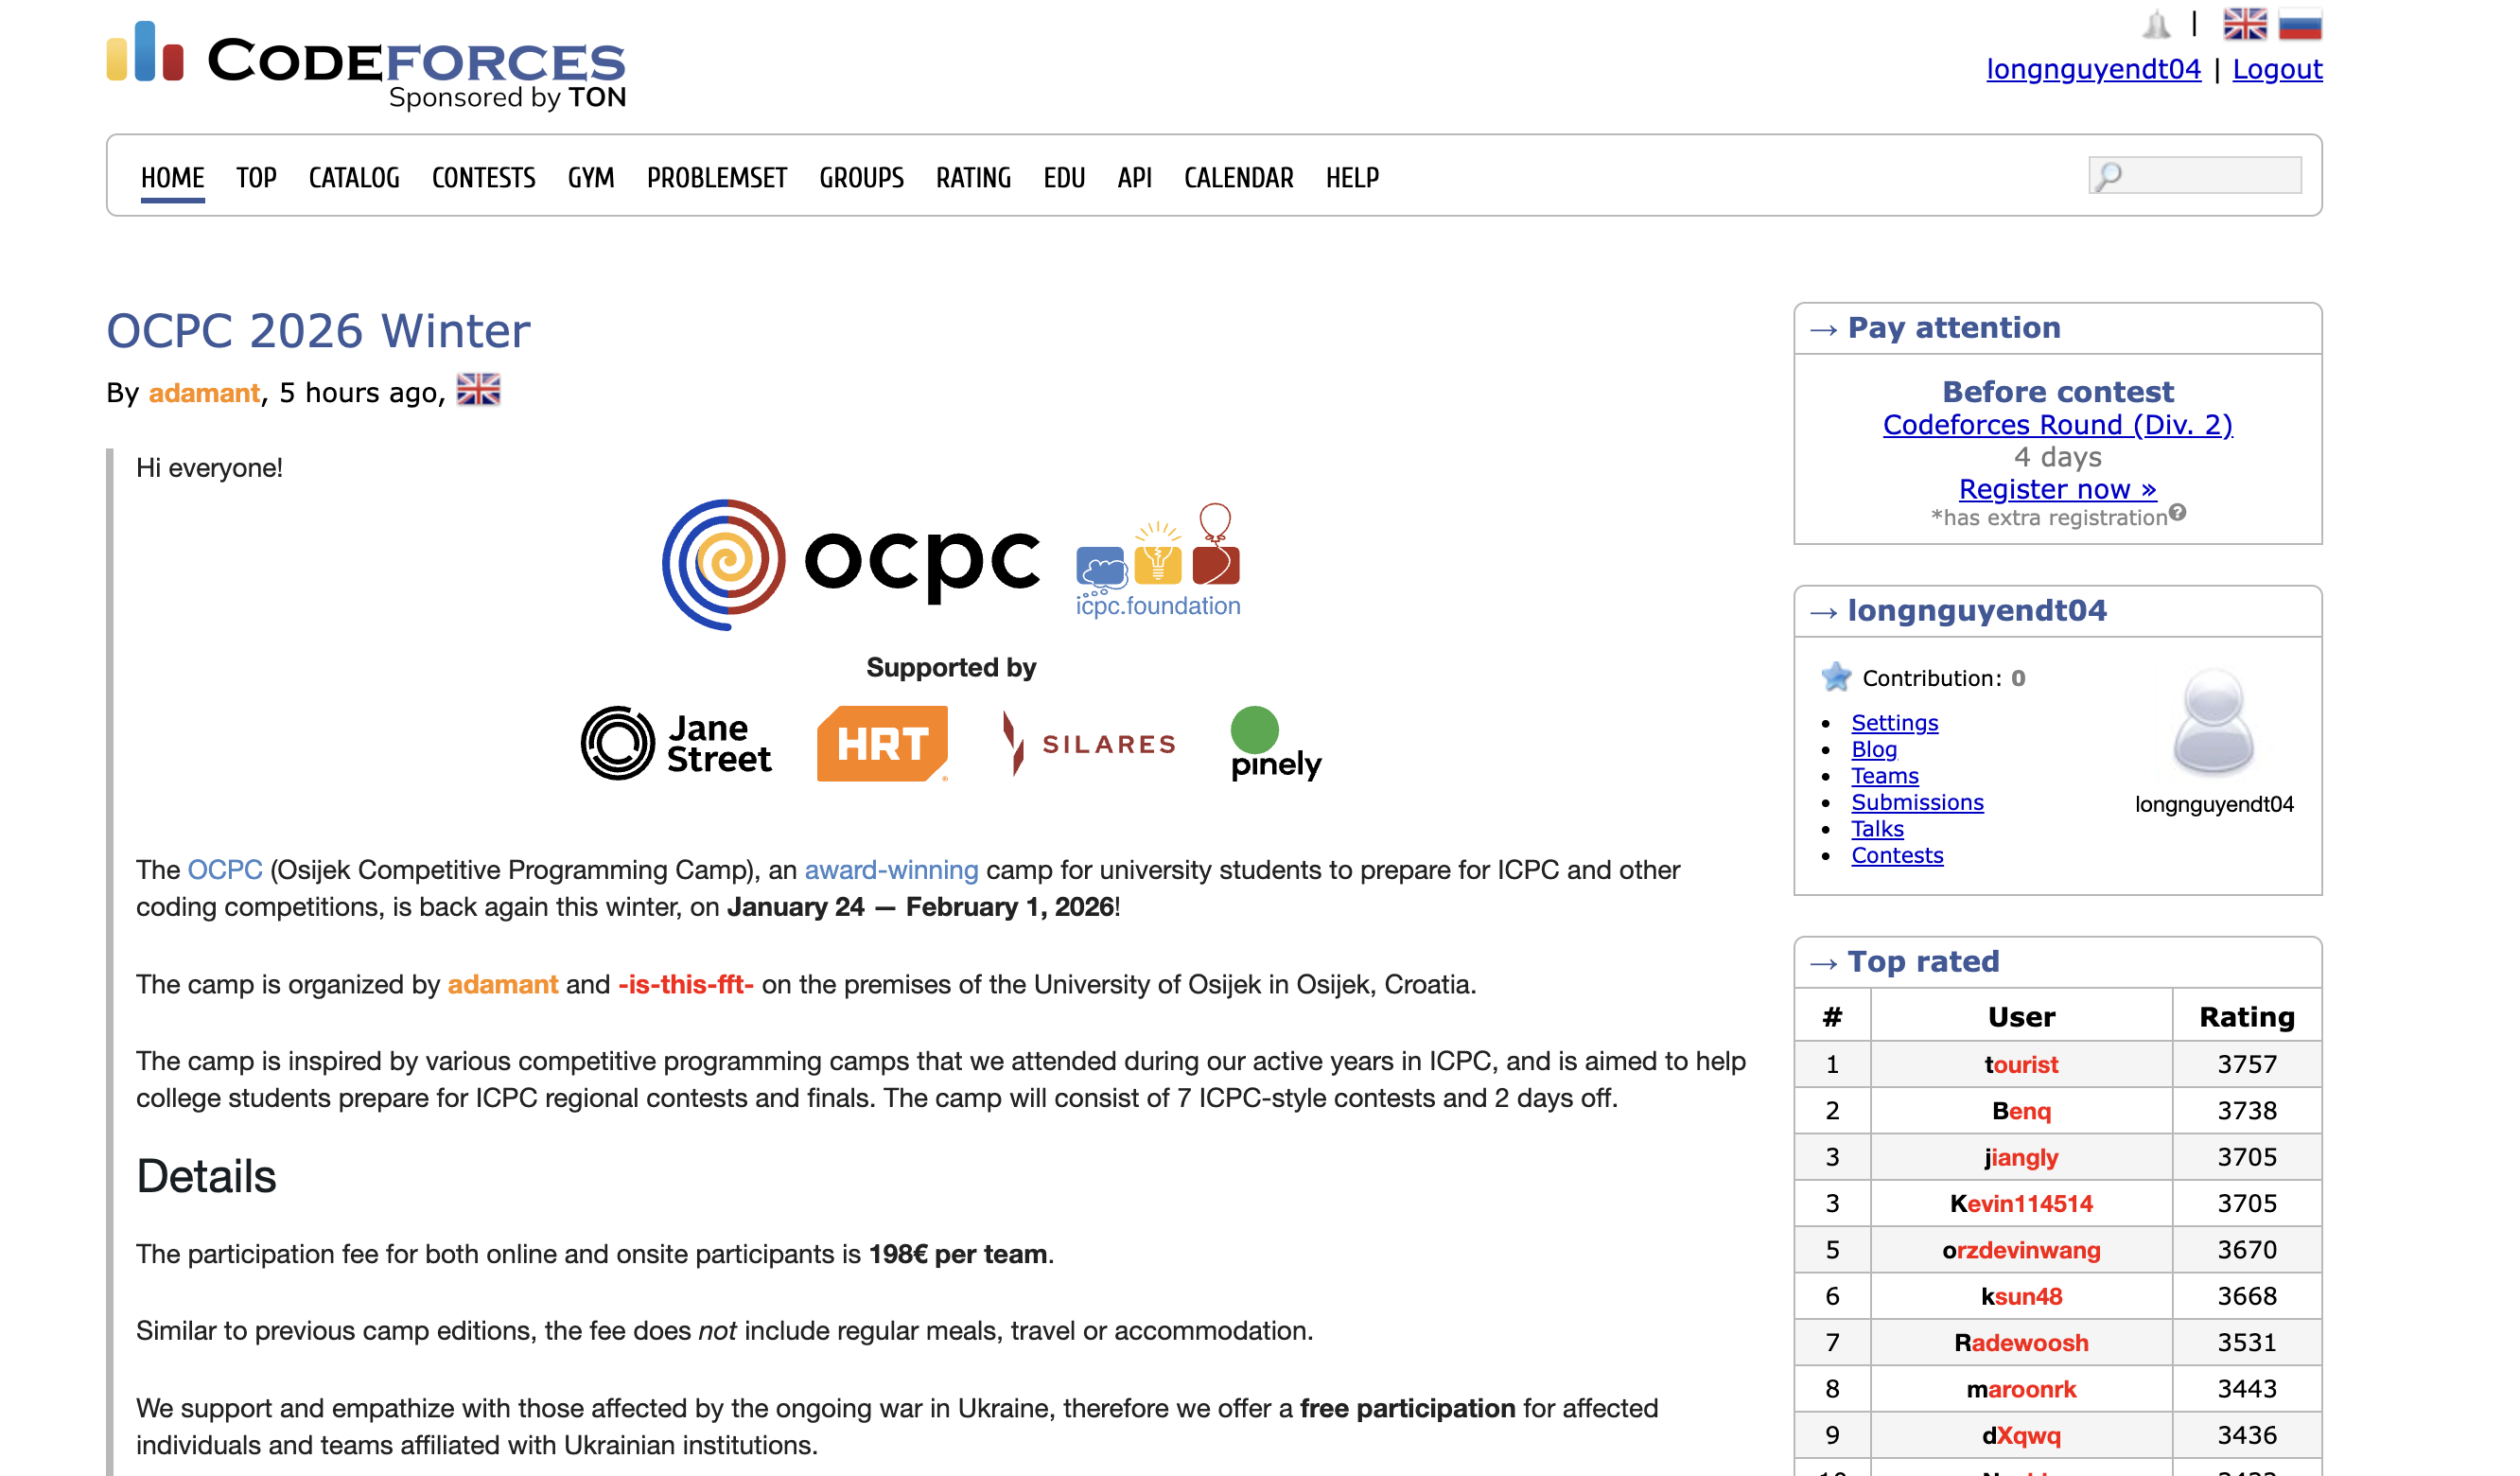
\includegraphics[width=1\textwidth]{Contents/Chapter 1/Images/Codeforces.png}
    \vspace{0.6cm}
    \caption{Codeforces Homepage}
    \label{fig:codeforces-system}
\end{figure}

Codeforces is a prominent online platform dedicated to competitive programming, offering users a structured environment to enhance their algorithmic and problem-solving skills through real-time contests. It is widely used by students, professionals, and competitive programmers to benchmark their abilities and engage with a global community of coders.\\

Key features of Codeforces include:
\begin{itemize}
    \item \textbf{Extensive Problem Sets:} A vast collection of algorithmic and programming problems across multiple difficulty levels.
    \item \textbf{Online Contests:} Regular timed competitions, including rated contests, that simulate real-world competitive programming scenarios.
    \item \textbf{Integrated Code Editor:} Supports multiple programming languages with submission, testing, and evaluation against problem test cases.
    \item \textbf{Community Discussion:} Active forums for problem discussions, solution sharing, and peer feedback.
    \item \textbf{User Ratings and Rankings:} Automatic rating system reflecting performance in contests and overall ranking among users globally.
    \item \textbf{Problem Tags and Difficulty Filters:} Tools to browse and search problems efficiently based on difficulty, topic, and tags.
\end{itemize}

Codeforces excels in providing a practical, competition-oriented environment that strengthens real-world programming and algorithmic skills. Its focus on timed contests and rigorous problem solving makes it an excellent platform for users aiming to improve performance in competitive programming. However, Codeforces does not currently provide dedicated tools for technical interview preparation, such as virtual assistants, hints, or structured interview question sets.

\subsection{VNOI Online Judge}

\begin{figure}[h!]
    \centering
    
\includegraphics[width=1\textwidth]{Contents/Chapter 1/Images/VNOI.png}
    \vspace{0.6cm}
    \caption{VNOI Online Judge Homepage}
    \label{fig:vnoi-system}
\end{figure}

VNOI Online Judge (VNOJ) is the official online judge system of the Vietnam Olympiad in Informatics community. The platform is based on the open-source DMOJ system and was built to provide a dedicated environment for Vietnamese learners to practice programming, compete in contests, and access problem sets from national and international competitions. VNOJ also continues the role of the former VOJ system by preserving and expanding a large archive of Vietnamese competitive programming problems.\\

Key features of VNOI Online Judge include:
\begin{itemize}
    \item \textbf{Vietnamese Problem Archive:} A large collection of problems from Vietnamese contests, national excellent student exams, ACM-ICPC style contests, and VNOI official events.
    \item \textbf{Automatic Online Judge:} Submission evaluation with verdicts, execution limits, and support for competitive programming workflows.
    \item \textbf{Contest System:} Official and practice contests organized for the Vietnamese competitive programming community.
    \item \textbf{User Ranking:} Public user profiles and ranking information that encourage competition and long-term practice.
    \item \textbf{Community Knowledge Base:} Links to VNOI Wiki, blogs, news, and learning resources focused on algorithms and programming contests.
    \item \textbf{Vietnamese Community Focus:} Content, announcements, and educational activities are tailored to Vietnamese students and competitive programmers.
\end{itemize}

VNOI Online Judge is especially valuable for Vietnamese IT students because it provides localized content, familiar contest formats, and access to problem sets from domestic competitions. Its strengths are closely aligned with competitive programming education and community development in Vietnam. However, VNOJ focuses mainly on algorithm practice and contest participation, while CodeRank aims to combine these competitive features with broader learning support such as interview preparation, centralized real-time discussions, and customizable user-created contests.

\subsection{ Websites comparison}
\begin{table}[h!]
\centering
\renewcommand{\arraystretch}{1.3}
\caption{Comparison of existing website with CodeRank}
\label{tab:website-comparison}
\begin{tabularx}{\textwidth}{|l|X|X|X|X|}
\hline
\textbf{Criteria} & \textbf{LeetCode} & \textbf{Codeforces} & \textbf{VNOI Online Judge} & \textbf{CodeRank} \\
\hline
Problem Library & Yes & Yes & Yes & Yes \\
\hline
Online Coding Editor & Yes & Yes & Yes & Yes \\
\hline
Community & Active discussion forums & Active forums with contest discussions & Vietnamese competitive programming community, blogs, wiki, and announcements & Centralized real-time discussion forums \\
\hline
Contest System & Regular contests organized by platform & Timed contests with system-created schedule & Official and practice contests for the VNOI community & Both official and user-created contests, customizable by users. \\
\hline
Interview Preparation & Yes & No & No & Yes \\
\hline
Ranking System & Points for solved problems, but not visible to all users & Rating system based on contest performance & Public user rankings and contest standings & Dynamic points for problem solving and public centralized leaderboard \\
\hline
Multilingual & Support English \& Chinese & Support English \& Russian & Mainly Vietnamese with some English problem content & Support English \& Vietnamese \\
\hline
\end{tabularx}
\end{table}

\FloatBarrier

Obviously, each platform has its own strengths: LeetCode offers an extensive problem library and dedicated interview preparation resources, Codeforces emphasizes timed contests, rating systems, and community-driven forums for competitive practice, and VNOI Online Judge provides localized Vietnamese problem sets, contests, and learning resources for the national competitive programming community. However, CodeRank combines these advantages and adds key enhancements, including both official and user-created contests with customizable settings, a centralized public leaderboard, real-time discussion forums, and multilingual support (including Vietnamese). These features make CodeRank a comprehensive, user-centered platform tailored to the educational and practical needs of Vietnamese IT students.

\newpage
